\documentclass{article}


\title{dag_drawing_pres}

\usepackage{tikz}
\tikzset{> = stealth} % nicer looking arrows

\begin{document}

Drawing with Tikz

\section{Example 1}

\begin{center}
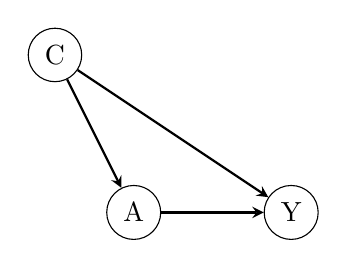
\begin{tikzpicture}
% nodes
\node[circle, draw] (C) at (0, 2) {C}; %create node, circle shape, named C with (X = 0, Y = 2) coordinates, labeled C
\node[circle, draw]  (A) at (1, 0) {A};
\node[circle, draw]  (Y) at (3, 0) {Y};
% edges
\draw[->, thick]
(C)	edge (A)
(C)	edge (Y)
(A)	edge (Y);

\end{tikzpicture}
\end{center}

\section{Example 2}

\begin{center}
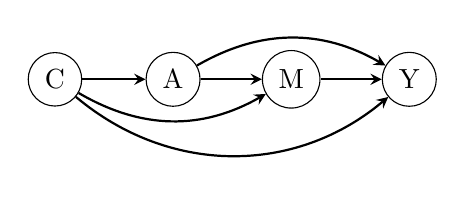
\begin{tikzpicture}
% nodes
\node[circle, draw] (C) at (0, 0)  {C}; %create node, circle shape, named C with (X = 0, Y = 2) coordinates, labeled C
\node[circle, draw]  (A) at (1.5, 0) {A};
\node[circle, draw]  (Y) at (4.5, 0) {Y};
\node[circle, draw] (M) at (3, 0) {M}; 
% edges
\draw[->, thick]
(C)	edge (A)
(C)	edge [bend right=40] (Y) % creating curve 
(C)	edge [bend right=30] (M)
(A)	edge [bend left=30] (Y)
(A)	edge (M)
(M)	edge (Y);

\end{tikzpicture}
\end{center}

\section{Example 3}

\begin{center}
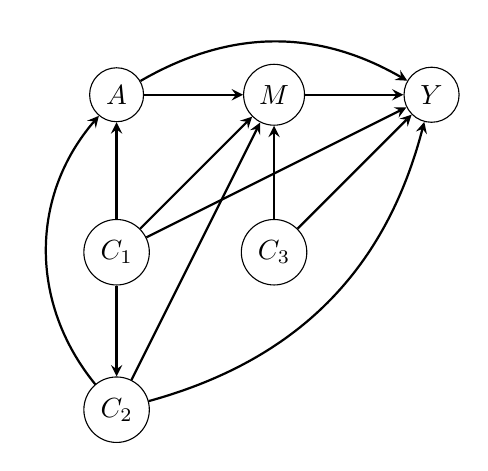
\begin{tikzpicture}
% nodes
\node[circle, draw] (C1) at (0, 2)  {$C_1$}; %create node, circle shape, named C with (X = 0, Y = 2) coordinates, labeled C
\node[circle, draw] (C2) at (0, 0)  {$C_2$}; % can use math mode to write labels!
\node[circle, draw] (C3) at (2, 2)  {$C_3$}; 
\node[circle, draw]  (A) at (0, 4) {$A$};
\node[circle, draw]  (Y) at (4, 4) {$Y$};
\node[circle, draw] (M) at (2, 4) {$M$}; 
% edges
\draw[->, thick]
(C1) edge (A)
(C1) edge (M)
(C1) edge (Y)
(C1) edge (C2)
(C2) edge [bend left=40] (A)  
(C2) edge (M) 
(C2) edge [bend right=30] (Y)
(C3) edge (M) 
(C3) edge (Y) 
(A)	edge [bend left=30] (Y)
(A)	edge (M)
(M)	edge (Y);

\end{tikzpicture}
\end{center}

\end{document}
